\section{Laplace Transformation}
\definition{Motivation}{Eine Transformation ermöglicht das Vereinfachen von 
Problemlösungen, indem das Problem in einem anderen 'Raum' gelöst wird.}

Beispiel:
\begin{equation*}
    \int \frac{x}{x^2+1} \text{d}x
\end{equation*}
Transformation: 
\begin{equation*}
    u = x^2 + 1 \Rightarrow \frac{\text{d}u}{\text{d}x}=2x\Rightarrow
    \text{d}x = \frac{\text{d}u}{2x}
\end{equation*}
Lösen:
\begin{equation*}
    \int \frac{1}{2u} \text{d}u = \frac{1}{2} \ln u
\end{equation*}
Rücktransformation:
\begin{equation*}
    \frac{1}{2} \ln \left( x^2+1 \right)
\end{equation*}

Der Laplace-Raum ist ein Raum, in dem Differentialgleichungen sehr einfach zu
lösen sind.

\subsection{Definition}
Annahme: Funktionen $f(t)$ sind so, dass
\begin{equation*}
    f(t)=0, \hspace{1em} t\leq0
\end{equation*}
\begin{center}
    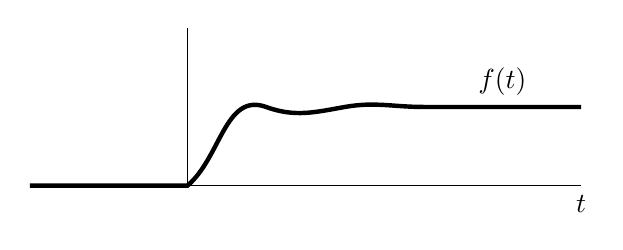
\begin{tikzpicture}
        \draw (0,2) -- (0,0) -- (5,0) node[below] {$t$};
        \draw[ultra thick] (-2,0) -- (0,0) 
            to[out=40,in=160] (1,1) 
            to[out=-20,in=190] (2,1)
            to[out=10,in=180] (3,1)
            -- (5,1) 
            node[pos=0.5,above] {$f(t)$};
    \end{tikzpicture}
\end{center}
\definition{Definition}{Laplace Transformation von $f(t)$}
\begin{equation*}
    \boxed{
        F(s) = \int_0^\infty f(t) e^{-st}\text{d}t
    }
\end{equation*}

Schreibweise:
\begin{eqnarr}
    F(s) &=&  \L (f(t)) \\
    F\tikzmark{a}(s) &\multimapdotbothB& f\tikzmark{b}(t)
\end{eqnarr}
\begin{center}
    \begin{tikzpicture}[overlay,remember picture]
        \node at (-2,0) (ta) {Bildfunktion};
        \node at (2,0) (tb) {Originalfunktion};
        \draw[->,thick] (ta) to (a);
        \draw[->,thick] (tb) to (b);
    \end{tikzpicture}
\end{center}

\bsp{Beispiele:}

\underline{Sprungfunktion}
\begin{equation*}
    \sigma (t) = \left\{ \begin{array}{c} 
            0 \text{ für } t<0\\
            1 \text{ für } t\geq0\\
    \end{array} \right.
\end{equation*}
\begin{center}
    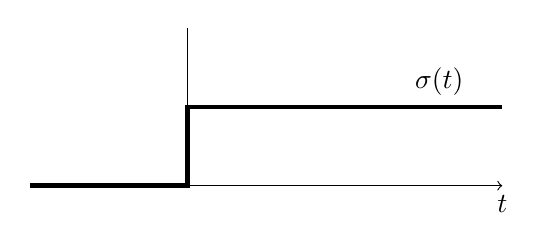
\begin{tikzpicture}
        \draw[->] (0,2) -- (0,0) -- (4,0) node[below] {$t$};
        \draw[ultra thick] (-2,0) -- (0,0) -- (0,1) -- (4,1)
            node[pos=0.8,above] {$\sigma(t)$};
    \end{tikzpicture}
\end{center}
\begin{eqnarr}
    \L \left( \sigma(t) \right) &=& \int_0^\infty e^{-st}dt \\
    &=&  \left. -\frac{1}{s} e^{-st}\right|_0^\infty \\
        &=& \frac{1}{s} \hspace{4em} \text{(falls Re} (s)>0)
\end{eqnarr}
\begin{equation*}
    \boxed{
        \frac{1}{s} \multimapdotbothB 1
    }
\end{equation*}

\underline{Lineare Funktion}
\begin{equation*}
    \sigma (t) = \left\{ \begin{array}{c} 
            0 \text{ für } t<0\\
            t \text{ für } t\geq0\\
    \end{array} \right.
\end{equation*}
\begin{center}
    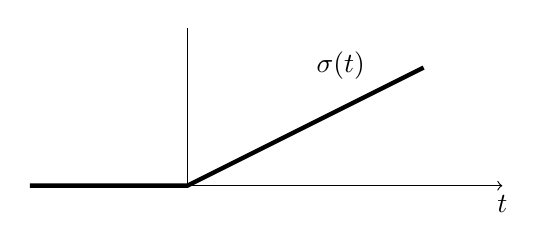
\begin{tikzpicture}
        \draw[->] (0,2) -- (0,0) -- (4,0) node[below] {$t$};
        \draw[ultra thick] (-2,0) -- (0,0) -- (3,1.5)
            node[pos=0.8,above left] {$\sigma(t)$};
    \end{tikzpicture}
\end{center}
\begin{eqnarr}
    \L \left( \sigma(t) \right) &=& \int_0^\infty te^{-st}dt \\
    &=&  \left. \left(  -\frac{-st-1}{s^2}\right) e^{-st}\right|_0^\infty \\
        &=& \frac{1}{s^2}
\end{eqnarr}
\begin{equation*}
    \boxed{
        \frac{1}{s^2} \multimapdotbothB t
    }
\end{equation*}

\underline{Kosinus}
\begin{equation*}
    \sigma (t) = \left\{ \begin{array}{c} 
            0 \text{ für } t<0\\
            \cos(\alpha t) \text{ für } t\geq0\\
    \end{array} \right.
\end{equation*}
\begin{center}
    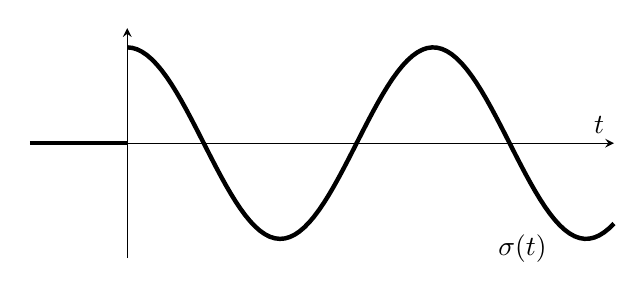
\begin{tikzpicture}
    \begin{axis}[
            width = 9cm,
            height = 4.5cm,
            axis lines = middle,
            clip = false,
            xmin = -2,
            ymin = -1.2,
            ymax = 1.2, 
            ticks=none,
            xlabel = $t$,
    ]
        \addplot[mark=none,samples=100,domain=0:10,ultra thick] {cos(deg(x))}
            node[pos=0.9,below left] {$\sigma(t)$};
        \draw[ultra thick] (axis cs:-2,0) -- (axis cs:0,0) ;
    \end{axis}
    \end{tikzpicture}
\end{center}
\begin{eqnarr}
    \L \left( \sigma(t) \right) &=& \int_0^\infty \cos(\alpha t)e^{-st}dt \\
    &\underset{\tiny{(324)}}{=}&  \left.   
        \frac{e^{-st}}{s^2+\alpha^2} \left[ -s \cos(\alpha t) + \alpha
        \sin(\alpha t) \right]
        \right|_0^\infty \\
        &=& -\frac{1}{s^2+\alpha^2}\left( -s \right)\\
        &=& \frac{s}{s^2+\alpha^2}
\end{eqnarr}
\begin{equation*}
    \boxed{
        \frac{s}{s^2+\alpha^2} \multimapdotbothB \cos(\alpha t)
    }
\end{equation*}

\subsection{Eigenschaften der Laplace Transformation}
\subsubsection*{Linearitätssatz}
\begin{equation*}
    \boxed{
        \L \left[ C_1f_1(t)+C_2f_2(t) \right] = 
        C_1\L\left[ f_1(t) \right] + C_2\L\left[ f_2(t) \right]
    }
\end{equation*}

\bsp{Beispiel}
\begin{eqnarr}
    f(t) &=&  3t^2-2t\\
    \L \left[ 3t^2-2t \right] &=& 3\L\left[ t^2 \right]-2\L[t]\\
    &=& 3\frac{2}{s^3}-2\frac{1}{s^2}\\
    &=& \frac{6}{s^3}-\frac{2}{s^2}\\
\end{eqnarr}

\subsubsection*{Ähnlichkeitssatz}
\begin{center}
    \begin{tikzpicture}
    \begin{axis}[
            width = 6cm,
            height = 3cm,
            axis lines = middle,
            clip = false,
            xmin = -2,
            ymin = -1.2,
            ymax = 1.2, 
            ticks=none,
            xlabel = $t$,
    ]
        \addplot[mark=none,samples=100,domain=0:10,ultra thick] {cos(deg(x))}
            node[pos=0.9,below left] {$f(t)$};
        \draw[ultra thick] (axis cs:-2,0) -- (axis cs:0,0) ;

        \coordinate (a) at (axis cs:5,-2.5);
    \end{axis}
    \begin{axis}[
            at={(6cm,0)},
            width = 6cm,
            height = 3cm,
            axis lines = middle,
            clip = false,
            xmin = -2,
            ymin = -1.2,
            ymax = 1.2, 
            ticks=none,
            xlabel = $t$,
    ]
        \addplot[mark=none,samples=100,domain=0:10,ultra thick] {cos(deg(2*x))}
            node[pos=0.95,above] {$f(at)$};
        \draw[ultra thick] (axis cs:-2,0) -- (axis cs:0,0) ;

        \coordinate (b) at (axis cs:5,-2.5);
    \end{axis}

    \draw (a) circle[radius=0.1] ++ (0,-0.1) -- ++ (0,-1) coordinate (a2);
    \fill (a2) circle[radius=0.1] node [below,yshift=-5pt] {$F(s)$};

    \draw (b) circle[radius=0.1] ++ (0,-0.1) -- ++ (0,-1) coordinate (b2);
    \fill (b2) circle[radius=0.1] node [below,yshift=-5pt]
    {$\dfrac{1}{a}F\left( \dfrac{s}{a} \right)$};
    \end{tikzpicture}
\end{center}
\begin{equation*}
    \boxed{
        \L\left( f(at) \right) = \frac{1}{a}F\left( \frac{s}{a} \right)
        \text{, wobei } f(t) \multimapdotbothA F(s)
    }
\end{equation*}

\underline{Beweis}
\begin{eqnarr}
    \L\left[ f(at) \right] &=& \int_0^\infty f(at) e^{-st}\text{d}t \\
    &=& \int_0^\infty f(u) e^{-\frac{s}{a}u}\frac{\text{d}u}{a} 
    \hspace{2em} \text{mit } u=at,~\frac{\text{d}u}{\text{d}t}=a\\
    &=& \frac{1}{a} F\left( \frac{s}{a} \right)
\end{eqnarr}

\bsp{Beispiel}

Annahme: $\sin(t) \multimapdotbothA \frac{1}{s^2+1}$
Was ist $\L \left[ \sin(at) \right]$?
\begin{eqnarr}
    \L\left[ \sin(at) \right] &=&  \frac{1}{a} 
            \frac{1}{\left( \frac{s}{a} \right)^2+1}\\
    &=& \frac{1}{a}\frac{a^2}{s^2+a^2}\\
    &=& \frac{a}{s^2+a^2}\\
\end{eqnarr}

\subsubsection*{Verschiebungssatz}
(nach rechts)

\begin{center}
    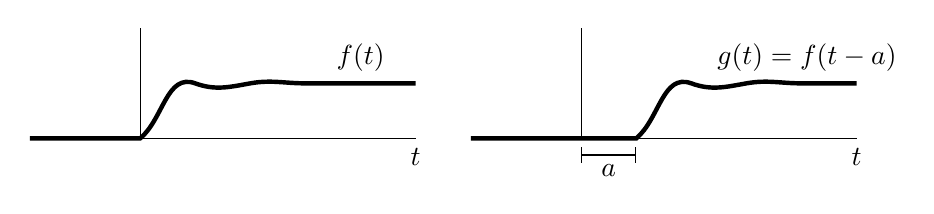
\begin{tikzpicture}[scale=0.7]
        \draw (0,2) -- (0,0) -- (5,0) node[below] {$t$};
        \draw[ultra thick] (-2,0) -- (0,0) 
            to[out=40,in=160] (1,1) 
            to[out=-20,in=190] (2,1)
            to[out=10,in=180] (3,1)
            -- (5,1) 
            node[pos=0.5,above] {$f(t)$};

        \draw (8,2) -- (8,0) -- (13,0) node[below] {$t$};
        \draw[ultra thick] (6,0) -- (9,0) 
            to[out=40,in=160] (10,1) 
            to[out=-20,in=190] (11,1)
            to[out=10,in=180] (12,1)
            -- (13,1)
            node[pos=0.1,above] {$g(t)=f(t-a)$};
            \draw[|-|] (8,-0.3) -- (9,-0.3) node[midway,below]{$a$};
    \end{tikzpicture}
\end{center}
\begin{equation*}
    \boxed{
        \L \left[ f(t-a) \right] = e^{-as}F(s),\hspace{1em}
        \text{wobei } f(t) \multimapdotbothA F(s), \hspace{1em} a>0
    }
\end{equation*}
\underline{Beweis}
\begin{eqnarr}
    \L \left[ f(t-a) \right] &=& \L\left[ \sigma(t-a) f(t-a)\right]\\
    &=& \int_a^\infty f(t-a)e^{-st}\text{d}t \hspace{2em} u=t-a\\
    &=& \int_0^\infty f(u) e^{-s(u+a)}\text{d}u\\
    &=& \int_0^\infty f(u) e^{-su}e^{-sa}\text{d}u\\
    &=& e^{-as}F(s)
\end{eqnarr}

\bsp{Beispiel}

\begin{center}
    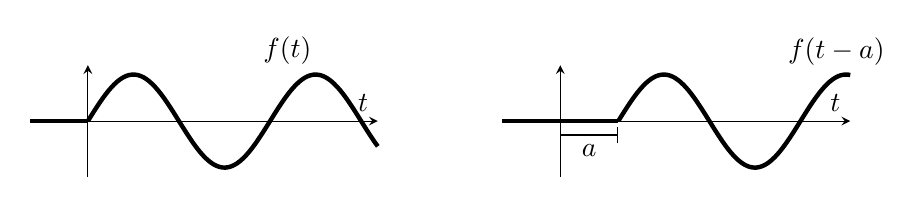
\begin{tikzpicture}
    \begin{axis}[
            width = 6cm,
            height = 3cm,
            axis lines = middle,
            clip = false,
            xmin = -2,
            ymin = -1.2,
            ymax = 1.2, 
            ticks=none,
            xlabel = $t$,
    ]
        \addplot[mark=none,samples=100,domain=0:10,ultra thick] {sin(deg(x))}
            node[pos=0.8,above left] {$f(t)$};
        \draw[ultra thick] (axis cs:-2,0) -- (axis cs:0,0) ;
    \end{axis}
    \begin{axis}[
            at={(6cm,0)},
            width = 6cm,
            height = 3cm,
            axis lines = middle,
            clip = false,
            xmin = -2,
            ymin = -1.2,
            ymax = 1.2, 
            ticks=none,
            xlabel = $t$,
    ]
        \addplot[mark=none,samples=100,domain=2:10,ultra thick] {sin(deg(x-2))}
            node[pos=0.95,above] {$f(t-a)$};
        \draw[ultra thick] (axis cs:-2,0) -- (axis cs:2,0) ;
        \draw[|-|] (axis cs:0,-0.3) -- (axis cs:2,-0.3) node[midway,below]{$a$};
    \end{axis}
    \end{tikzpicture}
\end{center}
Bekannt: \begin{equation*}
    \sin(t) \multimapdotbothA \frac{1}{s^2+1}
\end{equation*}
$\Rightarrow$
\begin{equation*}
    \L\left[ \sin(t-a) \right] = \frac{e^{-as}}{s^2+1}
\end{equation*}

\subsubsection*{Dämpfungssatz}
\begin{equation*}
    \boxed{
        \L\left[ e^{-at}f(t) \right] = F(s+a),
        \hspace{1em} \text{wobei }, f(t)\multimapdotbothA F(s)
    }
\end{equation*}
\underline{Beweis}
\begin{eqnarr}
    \L\left[ e^{-at}f(t) \right] &=& 
        e^{-at} \int_0^\infty f(t) e^{-st}\text{d}t\\
    &=& \int_0^\infty f(t) e^{-(s+a)t}\text{d}t\\
    &=& F(s+a)
\end{eqnarr}

\bsp{Beispiel}
\begin{eqnarr}
    1&\multimapdotbothA & \frac{1}{s}\\
    e^{-at}&\multimapdotbothA & \frac{1}{s+a}\\
\end{eqnarr}

\subsubsection*{Ableitungssatz}
\begin{eqnarr}
    f(t)&\multimapdotbothA&F(s)\\
    f'(t)&\multimapdotbothA&sF(s)-f(0)\\
    f''(t)&\multimapdotbothA&s^2F(s)-sf(0)-f'(0)\\
    f'''(t)&\multimapdotbothA&s^2F(s)-s^2f(0)-sf'(0)-f''(0)\\
    &\vdots&\\
    f^{(n)}(t)&\multimapdotbothA&s^nF(s)-s^{n-1}f(0)-s^{n-2}f'(0)
    \ldots -f^{(n-1)}(0)
\end{eqnarr}
\underline{Beweis} (für 1. Ableitung)
\begin{eqnarr}
    \L\left[ f'(t) \right] &=& \int_0^\infty \underbrace{f'(t)}_{u'}
    \underbrace{e^{-st}}_{v} \text{d}t \\
    &=& -\int_0^\infty f(t)(-s)e^{-st}\text{d}t+\left.f(t)\right|_0^\infty\\
    &=& s\int_0^\infty f(t)e^{-st}\text{d}t-f(0)\\
    &=& sF(s)-f(0)\\
\end{eqnarr}

\bsp{Beispiel}

Cosinusfunktion: $f(t)=\sin(t)$
\begin{equation*}
    \L[\cos(t)] = \L[f'(t)]=s\cdot \L[\sin(t)]-\underbrace{f(0)}_{=0}=
    \frac{s}{s^2+1}
\end{equation*}

\bsp{Beispiel}

Anfangswertproblem:
\begin{eqnarr}
    y'(t)+2y(t)&=& \sin(t), \hspace{1em} y(0)=1\\
    &&\\
    sY(s)-y(0)+2Y(s)&=& \frac{1}{s^2+1}\\
    Y(s)\left( s+2 \right)-1&=& \frac{1}{s^2+1}\\
    Y(s)\left( s+2 \right)&=& \frac{1}{s^2+1}+1\\
    Y(s)&=& \frac{1}{\left( s^2+1 \right)\left( s+2 \right)}+\frac{1}{s+2}\\
\end{eqnarr}
PBZ:
\begin{eqnarr}
    \frac{1}{\left( s^2+1 \right)\left( s+2 \right)} &=& 
      \frac{A}{s+2}+\frac{Bs+C}{s^2+1}\\
    1&=& As^2+A+Bs^2+2Bs+Cs+2C\\
    &&\\
    &&\left|
    \begin{array}{ccc} A+B&=& 0\\2B+C&=& 0\\2C+A&=& 1 \end{array}\right| \\
    &&\\
    &\Rightarrow& A=\frac{1}{5},~B=-\frac{1}{5},~C=\frac{2}{5}
\end{eqnarr}
\begin{eqnarr}
    Y(s)&=& \frac{0.2}{s+2}+\frac{-0.2s+0.4}{s^2+1}+\frac{1}{s+2}\\
    &=& \frac{1.2}{s+2}+\frac{-0.2s}{s^2+1}+\frac{0.4}{s^2+1}\\
    &\Rightarrow&\\
    y(t)&=& 1.2e^{-2t}-0.2\cos(t)+0.4\sin(t)\\
\end{eqnarr}

\subsubsection*{Integralsatz}
\begin{equation*}
    \boxed{
        \L\left[ \int_0^t f(\tau)\text{d}\tau \right] = \frac{1}{s} F(s)
        \text{ mit } f(t)\multimapdotbothA F(s)
    }
\end{equation*}
\bsp{Beispiel}

Bekannt: $t\multimapdotbothA\frac{1}{s^2}$, gesucht: $\L\left[ t^2 \right]$
\begin{eqnarr}
    \L\left[ t^2 \right] &=& \L\left[ \int_0^t 2\tau\text{d}\tau \right]\\
    &=& \frac{1}{s}\L\left[ 2t \right]\\
    &=& \frac{2}{s^3}
\end{eqnarr}

\subsection{Lösungen von DGL mit Laplace-Transformation}
\begin{outline}
    \1 Nur linear mit konstanten Koeffizienten. (Ordnung egal)
    \1 Mit Anfangswerten
\end{outline}

Idee:

\begin{center}
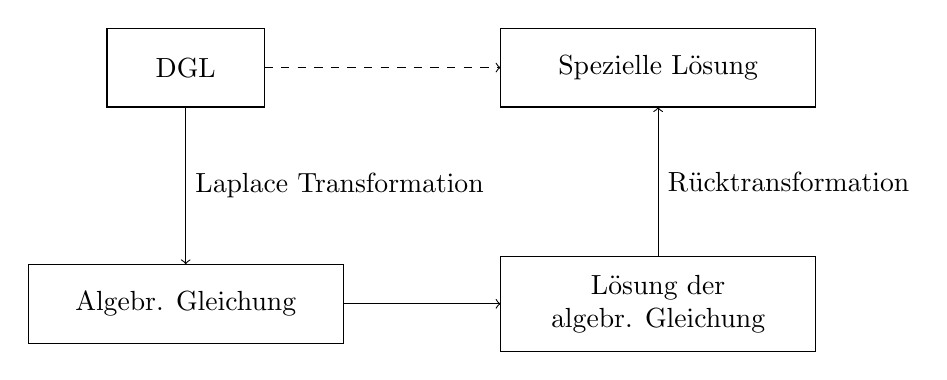
\begin{tikzpicture}
    \draw (1,0) rectangle ++(2,1) node[midway] {DGL};
    \draw (0,-3) rectangle ++(4,1) node[midway] {Algebr. Gleichung};
    \draw (6,0) rectangle ++(4,1) node[midway] {Spezielle Lösung};
    \draw (6,-3.1) rectangle ++(4,1.2)
        node[midway,align=center] {Lösung der \\algebr. Gleichung};

    \draw[->] (2,0) -- ++(0,-2) node[midway,right] {Laplace Transformation};
    \draw[->] (4,-2.5) --++ (2,0);
    \draw[->] (8,-1.9) --++ (0,1.9) node[midway,right] {Rücktransformation};
    \draw[dashed,->] (3,0.5) --++ (3,0);
\end{tikzpicture}
\end{center}

\bsp{Beispiel}
\begin{equation*}
    y''+2y'+y=9e^{2t}, \hspace{1em} y(0)=0,~y'(0)=1
\end{equation*}
Lösen mit Laplace:
\begin{eqnarr}
    \left[ s^2Y(s)-s\cdot 0-1 \right]+2\left[ sY(s)-0 \right] + Y(s)
    &=& \frac{9}{s-2}\\
    Y(s)\left[ s^2+2s+1 \right] &=& \frac{9}{s-2}+1\\
    Y(s)&=& \frac{s+7}{\left( s-2 \right)\left( s^2+2s+1 \right)}\\
        &=& \frac{s+7}{\left( s-2 \right)\left( s+1 \right)^2}\\
\end{eqnarr}
PBZ:
\begin{eqnarr}
     \frac{s+7}{\left( s-2 \right)\left( s+1 \right)^2}
     &=& \frac{A}{s+1}+\frac{B}{\left( s+1 \right)^2}+\frac{C}{s-2}\\
     s+7&=& A\left( s+1 \right)\left( s-2 \right)+B(s-2)+C\left( s+1 \right)^2\\
      &=& As^2-As-2A + Bs-2B+Cs^2+2Cs+C\\
      &&\\
    &&\left|
    \begin{array}{ccc} A+C&=& 0\\-A+B+2C&=& 1\\-2A-2B+C&=& 7 \end{array}
    \right| \\
    &&\\
    && A=-1,~B=-2,~C=1
\end{eqnarr}
Rücktransformieren:
\begin{eqnarr}
    \frac{s+7}{\left( s-2 \right)\left( s+1 \right)^2} &=& 
        -\frac{1}{s+2}-\frac{2}{\left( s+1 \right)^2}+\frac{1}{s-2}\\
    y(t)&=& \L^{-1}\left[-\frac{1}{s+2}-\frac{2}{\left( s+1
    \right)^2}+\frac{1}{s-2}\right]\\
    &=& -\L^{-1}\left[\frac{1}{s+2}\right]-2\L^{-1}\left[\frac{1}{\left( s+1
    \right)^2}\right]+\L^{-1}\left[\frac{1}{s-2}\right]\\
        &=& -e^{-t}-2te^{-t}+e^{2t}
\end{eqnarr}
